\documentclass[12pt,a5paper]{article}

\usepackage[T1]{fontenc} % font encoding, lubab õ tähte kasutada
\usepackage[utf8]{inputenc} % oleme siiski 21. sajandis, vajadusel on ka olemas utf8x
\usepackage{lmodern} % lmodern ja micrtype käivad käsikäes, teeb teksti ilusamaks
\usepackage{tikz}
\usetikzlibrary{decorations.pathreplacing, positioning}
\usepackage{microtype}
\usepackage[estonian]{babel} % eesti keele poolitamisreeglid jpm
\usepackage[per = fraction, expproduct=cdot, decimalsymbol=comma]{siunitx} % http://www.bakoma-tex.com/doc/latex/siunitx/siunitx.pdf
\usepackage{graphicx} 
\usepackage{wrapfig}
\usepackage{epstopdf} %minul on vaja, et .eps pilte saada
\usepackage{icomma} %koma arvust mõistlikul kaugusel
\usepackage{amsmath}
\usepackage{enumitem}
\usepackage{caption}
\usepackage{pgfplots}
\usepackage{float}

\special{papersize=14.85cm,21cm}

%paneme kõik mõõdud paika
\topmargin=-2.5cm \textheight=18.5cm \textwidth=12.77cm
\oddsidemargin=-1.5cm  \evensidemargin=-1.5cm
\setlength{\parindent}{0pt} \setlength{\parskip}{6pt} \sloppy

\relpenalty=10000 \binoppenalty=10000 % Tekstisisestes valemites reavahetusi ärgu olgu


\pagestyle{empty} % ilma leheküljenumbrita

\newcommand{\numb}[1]{\vspace{5pt}\textbf{\large #1}}
\newcommand{\nimi}[1]{(\textsl{\small #1})}
\newcommand{\punktid}[1]{(\emph{#1~p.})}
\newcounter{ylesanne}
\newcommand{\yl}[1]{\addtocounter{ylesanne}{1}\numb{\theylesanne.} \nimi{#1} \newblock{}}
\newcommand{\pp}[1]{[\textbf{#1~p.}]}
\newcommand{\pv}[1]{\quad \hbox{[\textbf{#1~p.}]}}
\newcommand{\ue}[1]{\underline{\emph{#1}}}
\newcommand{\hence}{\quad \Rightarrow \quad}
\newcommand{\autor}[1]{\emph{ Autor: #1.\\}}


\begin{document}

\begin{center}
\textbf{\Large Eesti koolinoorte 65. füüsikaolümpiaad} \vspace{2pt}

\emph{19. jaanuar 2019. a. Piirkondlik voor.}

\emph{{\bf Gümnaasiumi} ülesannete lahendused}


\end{center}

\numb{Eessõna}

Allpool on toodud iga ülesande üks õige lahenduskäik (mõnel juhul ka
enam). \textbf{Kõik alternatiivsed õiged lahenduskäigud tuleb hinnata samuti maksimumhindega.} Iga alternatiivse lahenduskäigu jaoks tuleb
kontrollijatel koostada hindamisskeem, juhindudes võimalusel juuresoleva
hindamisskeemi punktijagamisproportsioonist. Soovituslikud
maha-arvamise punktid: numbriline arvutusviga --- 0,5; viga
teisendustes --- 0,5 p. (märgi jms väiksem viga) või 1 p. (viga, mis
viib dimensioonide konf\/liktini), maha arvata ainult üks kord, st
edasikanduvat viga mitte karistada; kui vastus tuleb füüsikaliselt
absurdne, siis võib täiendavalt karistada 0,5 punktiga; üksik viga
lähtevalemis: 0,5 p. (kui märgiviga), kuni 50\% (sisuline viga).

\yl{RONG} \punktid{6} \autor{Carel Kuusk}
Olgu rongi kiirendus $a$. Kuna vagunid on identsed, siis ühe vaguni pikkus $s=\frac{at^2}{2}$. \pp{1} Olgu rongis $n$ vagunit, siis kõik vagunid mööduvad Jukust 
aja $t_n=\sqrt{\frac{2sn}{a}}$ jooksul. \pp{1} Kõik peale viimase vaguni mööduvad aja $t_{n-1}=\sqrt{\frac{2s(n-1)}{a}}$ jooksul. \pp{1} Seega 
$$t_2=t_n-t_{n-1}=\sqrt{\frac{2sn}{a}}-\sqrt{\frac{2s(n-1)}{a}}=t(\sqrt{n}-\sqrt{n-1}) \quad \pp{1}$$
Siit tuleb ruutvõrrand, mille lahendades saame:
$$n = \frac{1}{4}\bigg(\frac{t_2}{t}\bigg)^2 + \frac{1}{2} + \bigg(\frac{t}{4t_2}\bigg)^2 = 7.97 \approx 8 \quad \pp{1}$$
Üle kontrollides ainuke antud vahemikku sobiv $n=8$ \pp{1}. 

\newpage
\yl{PEEGEL} \punktid{6}\autor{Jaan Kalda}
Paneme tähele, et ükski kiirefragment ei ole teisega samal sirgel \pp{1}. See tähendab, et kõikide kiirefragmentide puhul on tegemist kas erinevate kiirtega või sama kiire fragmentidega enne ja pörast peegeldumist \pp{1}. Et kiiri on kokku ainult kolm, siis vähemalt kaks fragmenti peavad olema pärit samalt kiirelt, üks enne ning teine pärast peegeldumist \pp{1}. Kui me suudame kindlaks teha, millised on need kaks fragmendipaari, siis saame leida peegli asukoha kui kahe kiirepaari pikenduste lõikepunkte ühendava joone. Viis fragmenti annavad pikendades viis sirget, mis lõikuvad paarikaupa kümnes erinevas punktis. Pikendame kõiki kiiri lõikumisteni ja leiame need 10 lõikepunkti (9-10 lõikepunkti: \pp{1}; 8 või vähem lõikepunkti: \pp{0} punkti). Ühendame need 15 lõikepunktipaari, mida ühendav joon saab olla peegliks (st mis ei ole juba ühendatud fragmendipikendusega), joonega (punased jooned joonisel) (11-15 joont: \pp{1}; 10 või vähem joont: \pp{0}). Leiame punaste joonte hulgast sellise, mis sobib peegliks: joon moodustab vastavalt võrdsed nurgad lõikuvate kiirtega, (joonisel on võrdsed nurgad märgitud roheliste ja siniste kaarekestega ning peegli asukoht jämeda punase joonega) \pp{1}. 
\begin{center}
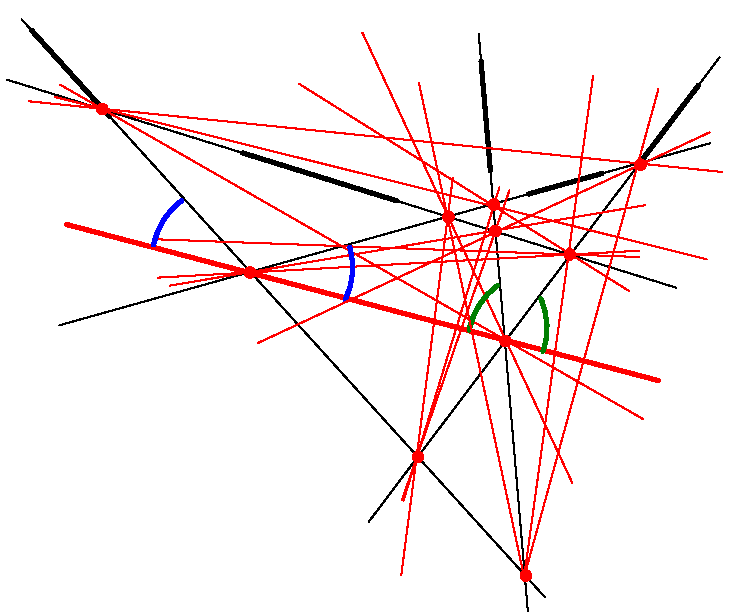
\includegraphics[scale=0.7]{peegel_lah.pdf}
\end{center}
\newpage
\yl{KÄRBES LENDAB}\punktid{8}\autor{Erkki Tempel}
  \vspace{-20pt}
  \begin{center}
    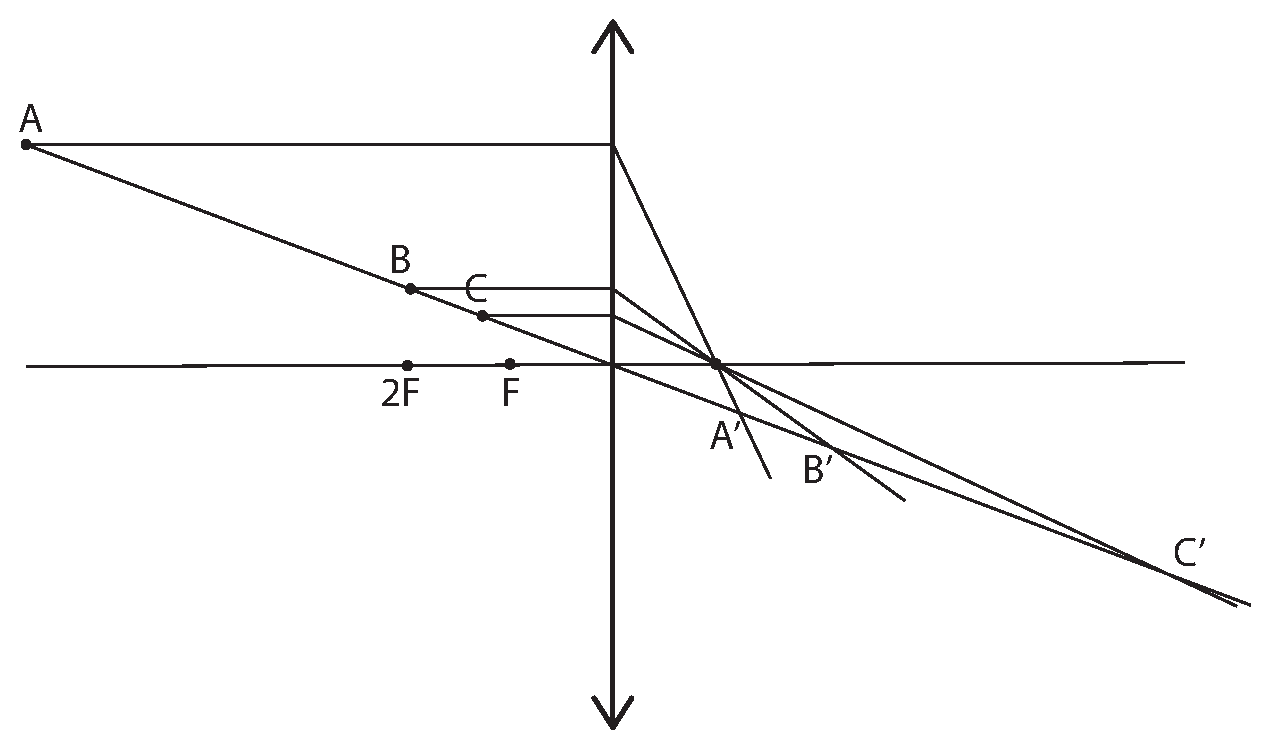
\includegraphics[width=0.7\textwidth]{karbeslah}
  \end{center}
  \vspace{-20pt}


Kuna kärbes lendab otse oma kujutise poole, siis peab ta lendama läätse keskpunkti poole, seega kärbes ja tema kujutis asuvad alati sirgel $AC'$. \pp{1}\\ 
Kui kärbes lendab punktist $A$ punkti $B$, siis kujutis liigub punktist $A'$ punkti $B'$. Jooniselt on näha, et kärbse kujutis liigub aeglasemalt kui kärbes. Konstrueerides punktide $A$ ja $B$ vahele veel punkte on näha, et kujutise kiirus on järjest suureneb, kui kärbes läheneb punktile $B$. \pp{2}\\
Kui kärbes asub läätsest kahekordse fookuskauguse kaugusel (punkt $B$), siis asub ka kujutis läätsest kahekordse fookuskauguse kaugusel (punkt $B'$). \pp{1} Sellises kohas on kärbse ja tema kujutise kiirused võrdsed, seega on kärbse ja tema kujutise kiirus teineteise suhtes $v_{min} = \SI{0}{m/s}$. \pp{1}\\
Kui kärbes liigub punktist $B$ fookaaltasandi suunas, siis kujutise kiirus järjest suureneb \pp{1} ning vahetult enne fokaaltasandile jõudmist on kujutise kiirus lõpmatult suur ($v_{max} \rightarrow \infty\SI{}{\,m/s}$) \pp{1}. Seega on kujutise kiirus kärbse suhtes maksimaalne siis, kui kärbes on väga lähedal fokaaltasandile ehk kärbes asub läätse tasandist fookuskauguse kaugusel. \pp{1} 


\yl{VAAKUM} \punktid{8} \autor{Valter Kiisk}
\osa Toru tühjakspumpamine tähendab sisuliselt õhu väljasurumist torust, tehes tööd välisrõhu $p$ vastu. \pp{1} Õhk mõjub kuulikesele resultatiivse jõuga $pS$, kus toru ristlõikepindala $S=\pi(d/2)^2=\SI{0.79}{cm^2}$. \pp{1} Jõudu $pS$ tuleb rakendada teepikkusel $\ell$, nii et tehtud töö $A=pS\ell$. \pp{1}   $A=\SI{101300}{Pa}\cdot \SI{7.9e-5}{m^2}\cdot\SI{1}{m}\approx\SI{8.0}{J}$. \\
\osa Kuulikese mass: \[m=\rho V=\rho(4/3)\pi(d/2)^3=\pi \rho d^3/6= \pi\cdot \SI{7.9}{g/cm^3}\cdot (\SI{1}{cm})^3/6 =\SI{4.1}{g}\] \pp{1} Kuna kuulike liigub eeldatavasti hulga aeglasemalt kui on heli kiirus, siis talle mõjub praktiliselt konstantne kiirendav jõud $pS$, jällegi teepikkusel $\ell$. Järelikult eelmises punktis leitud töö $A$ annab ühtlasi kuulikese kineetilise energia toru teises otsas. \pp{1} Kuna $mv^2/2=A$, siis $v=\sqrt{2A/m}$. \pp{1}
\[
v=\sqrt{\frac{2\times \SI{8.0}{J}}{\SI{0.0041}{kg}}}\approx\SI{62}{m/s}\,\text{\pp{1}}
\]
Alternatiivselt võib kasutada ka tuntud valemit ühtlase kiirenduse jaoks, $v^2-v_0^2=2a\ell$, kus algkiirus $v_0=0$ ja kiirendus $a=pS/m$.
	

\yl{OSAKE MAGNETVÄLJAS} \punktid{8} \autor{Erkki Tempel}
Kui osake siseneb magnetvälja, siis mõjub osakesele Lorenzi jõud $F_L = qvB\sin{\alpha}$ \pp{1}. Osake siseneb magnetvälja risti magnetväljaga ning hakkab Lorentzi jõi tõttu liikuma mööda ringjoont. \pp{2}

Ringjoone raadius $r$ on minimaalne siis, kui osake siseneb magnetvälja alt ning väljub ülevalt servast. Mööda ringjoont liikudes mõjub osakesele tsentrifugaaljõud
\[ F_T = \frac{mv^2}{r} \quad\quad\pp{1} \]
Lorentzi jõud ja tsentrifugaaljõud on võrdsed \pp{1}, seega saame avaldada ringjoone raadiuse $r$
\[ F_L = F_T \quad\quad\Rightarrow\quad\quad qvB = \frac{mv^2}{r} \quad\quad\Rightarrow\quad\quad r = \frac{mv^2}{qvB} \quad\quad\pp{2}\]
Seega on magnetvälja ala minimaalne laius $l$
\[ l = 2r = \frac{2mv^2}{qvB} \quad\quad\pp{1} \]

 \vspace{-20pt}
  \begin{center}
    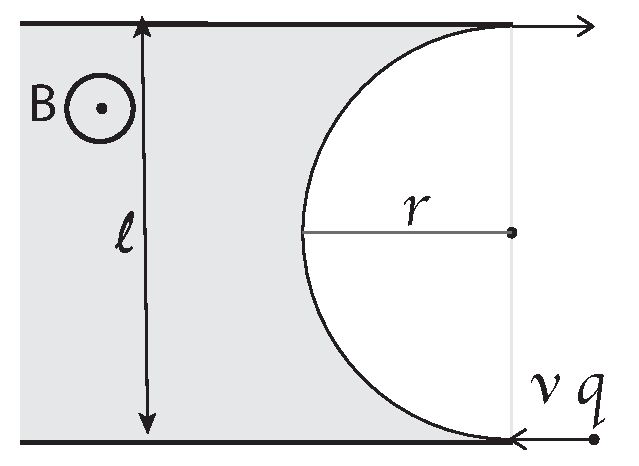
\includegraphics[width=0.5\textwidth]{osakelah}
  \end{center}
  \vspace{-20pt}

\yl{KONDENSAATOR} \punktid{8} \autor{Hans Daniel Kaimre}
Pinge kondensaatoril on  maksimaalne, kui see on täis laetud \pp{1}. Sellisel juhul kondensaatorit ning ka takistit $R_3$ vool ei läbi \pp{1} ning omakorda pingelang takistil $R_3$ on null \pp{1}. See tähendab, et pinge kondensaatori klemmidel on võrdne pingega takistil $R_2$. \pp{2} Viimase saamegi leida Ohmi seadusest:
$$U_2=I_2R_2 \quad I_2=\frac{U}{R_1+R_2} \Rightarrow U_2=U_C=\frac{U}{R_1+R_2}R_2\quad\pp{2}$$
Asendame sisse teada olevad väärtused:
$$U_C=\frac{\SI{12}{\V}}{\SI{1}{\kilo\ohm}+\SI{2}{\kilo\ohm}}\cdot\SI{2}{\kilo\ohm}=\SI{8}{\V}\quad\pp{1}$$

\yl{LENNURADA} \punktid{8} \autor{Jonatan Kalmus}
Teame, et jõud on võrdeline õhu tiheduse ning kiiruse ruuduga. Seega olgu 
$$F=C\rho v^2 \Rightarrow v^2=\frac{F}{C\rho}$$
kus $C$ on võrdetegur. \pp{2} Kuna lennuk alustab hoovõttu paigalseisust ühtlase kiirendusega $a$, avaldub läbitud teepikkus $s=\frac{v^2}{2a}$. \pp{1} Kuna lennuki mass (ning seega ka õhkutõusuks vajaminev üleslükkejõud) ja kiirendus on mõlemal juhul samad \pp{1}, avalduvad teepikkused vastavalt:
$$s_1=\frac{v_1^2}{2a}=\frac{F}{2Ca\rho_1}\quad\pp{1}$$ 
$$s_2=\frac{v_2^2}{2a}=\frac{F}{2Ca\rho_2}\quad\pp{1}$$   

Võrrandid omavahel jagades saame:
$$\frac{s_1}{s_2}=\frac{\rho_2}{\rho_1}\quad\pp{1}$$ 
Siit saame avaldada vajaliku lennuraja pikkuse $s_2 = s_1\frac{\rho_1}{\rho_2} \approx \SI{3}{km}\quad  \pp{1}$.

\yl{GRANAAT} \punktid{12} \autor{Oleg Košik}
Granaadi vertikaalsuunaline algkiirus on $v_0=v\sin\alpha$ \pp{1}.

Kuna masskeskme süsteemis kaugenevad killud võrdse kiirusega $u$ keskpunktist, siis võime ette kujutada, et ajahetkel $t$ peale granaadi lõhkemist lendab ta edasi, kuid seda ümbritseb kildudest koosnev sfäär raadiusega $ut$ \pp{2}.

Seega kui esimene kild jõuab maapinaanni, on sfääri raadiuseks $u(t_2-t_1)$, ehk ajahetkel $t_2$ on sfääri keskpunkti kõrguseks $u(t_2-t_1)$ \pp{2}. Paneme tähele, et sfääri keskpunkt liigub nii, nagu oleks liikunud granaat, kui see ei oleks lõhkenud. Sfääri keskpunkti liikumisvõrrandist on selle lennukõrgus ajahetkel $t_2$ võrdne $h_2=v_0t_2-\frac{gt_2^2}{2}$ \pp{1}, ehk saame
$$
v_0t_2-\frac{gt_2^2}{2}=u(t_2-t_1). \pv1
$$
Selle võrrandi positiivne lahend on $t_2=\frac{(v_0-u)+\sqrt{(v_o-u)^2+2gt_1u}}{g}$ \pp{1}.

Kui viimane kild jõuab maapinaanni, on sfääri (mis nüüdseks on juba mõtteline, sest ülejäänud selle sfääri pinnal olevad killud lebavad maas) raadius $u(t_3-t_1)$. Seega, ajahetkel $t_3$ on meie mõttelise sfääri keskpunkt kõrgusel $h_3=-u(t_3-t_1)$ \pp{2}. See annab võrrandiks
$$
v_0t_3-\frac{gt_3^2}{2}=-u(t_3-t_1). \pv1	
$$
Pidades silmas, et $t_3>t_2$, saame selle lahendiks $t_3=\frac{v_0+u+\sqrt{(v_o+u)^2-2gt_1u}}{g}$ \pp{1}.

\yl{KIIK} \punktid{12} \autor{Jonatan Kalmus}	
\osa Minimaalne jõud: Haripunktis on Juku hetkeliselt vabalangemises ning mingit jõudu ei avalda. Seega on minimaalne jõud: 
$$F_{min} = 0 \quad\pp{1.5}$$ 
Maksimaalne jõud: Kiikumise ajal rakenduvad postidele 2 jõudu: Juku raskusjõud ning pöörlemisest tulev tsentrifugaaljõud. Mõlemad on maksimaalsed ning samasuunalised, kui kiik on vertikaalasendis \pp{0.5}. Olgu kiige pöörlemisraadius Juku masskeskme suhtes $R = H-h$. Kasutades energia jäävust kiige vertikaal- ja horisontaalasendi jaoks saame: 
$$mgR = \frac{mv^2}{2} \Rightarrow v^2 = 2gR \quad\pp{1}$$ 
Tsentrifugaaljõu valemist saame:
$$F_C = m\frac{v^2}{R} = m\frac{2gR}{R} = 2mg \quad\pp{1}$$ 
Summarne jõud:
$$F_{max} = F_C + F_R = 2mg + mg = 3mg \quad\pp{0.5}$$ 
\osa Minimaalne jõumoment: Kiige vertikaalasendis on jõuõlg kiigeposti alumise punkti suhtes $0$, seega minimaalne jõumoment:
$$\tau_{min} = 0\quad\pp{1}$$ 
Maksimaalne jõumoment: Kuna võll kõrgusel $H$ on ainuke kiige kinnituspunkt, rakendub kogu Juku poolt rakendatav jõud sellesse punkti \pp{0.5}. Jõumoment on maksimaalne, kui jõuõlg $H$ ning sellesse punkti rakenduv jõud on risti. Seega piisab maksimaalse horisontaalse jõu leidmisest. Tähistame kiige hetkeasukoha ja haripunkti tasandi vahelise kauguse $s$ ning nende vahelise nurga $\varphi$ (vt. joonis). Tsentrifugaaljõud on alati suunatud piki raadiust ning analoogselt maksimaalse jõu arvutusele saame energia jäävusest:
$$F_C = m\frac{2gs}{R} = 2mg\sin{\varphi}\quad\pp{1}$$ 
Lisaks tuleb arvestada raskusjõu raadiusesihilist komponenti $F_{R||} = F_R\sin{\varphi} = mg\sin{\varphi}\pp{1.5}*$.
Seega rakendub piki raadiust võllile jõud:
$$F_{||} = F_C + F_{R||} = 3mg\sin{\varphi}\quad\pp{0.5}*$$ 
Meid huvitab selle jõu horisontaalkomponent:
$$F_H = F_{||}\cos{\varphi} = 3mg\sin{\varphi}\cos{\varphi}\quad\pp{0.5}$$ 
Teades, et $\sin{2\varphi}=2\sin{\varphi}\cos{\varphi}$ saame:
$$F_H = \frac{3}{2}mg\sin{2\varphi}\quad\pp{1}$$ 
Siinuse maksimaalne väärtus on $1$, mille saame $\varphi = \ang{45}$ korral, mis on antud ülesande jaoks reaalne väärtus. Seega saame maksimaalseks horisontaalseks jõuks:
$$F_H = \frac{3}{2}mg\quad\pp{1}$$ 
Millele vastab maksimaalne jõumoment:
$$\tau_{max} = F_HH = \frac{3}{2}mgH\quad\pp{0.5}$$ 

Märkus: Kui õpilane jätab maksimaalse jõumomendi leidmisel arvestamata raskusjõuga, jääb saamata summarselt \pp{2} (1.5 + 0.5, märgitud tärniga).
\begin{center}
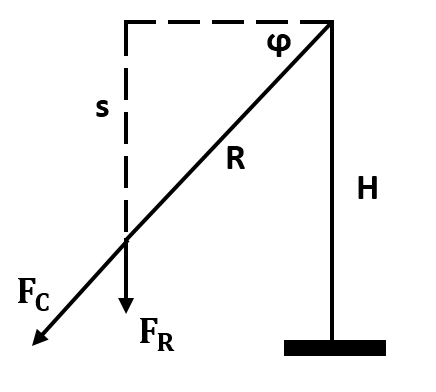
\includegraphics[scale=0.5]{Kiik.png}
\end{center}


\yl{3 DIOODI} \punktid{12} \autor{Jaan Kalda}
Lahendus. Vaatleme protsessi, kus sisendpinget hakatakse aeglaselt suurendama alates nullist. Väikese voolu korral on pingelang takisteil tühine, seetõttu on kõigi dioodide pinged peaaegu võrdsed. See tähendab, et esimesena avaneb kõige madalama avanemispingega diood - punane diood. Voolu kasvatamisel pingelang takisteil kasvab; et esialgu on roheline diood suletud, siis läbib mõlemat takistid sama tugev vool, mis tähendab et ka takistite pinged on võrdsed. Et rohelise ja punase dioodi avanemispingete vahe on suurem, kui sinise ja rohelise dioodi avanemispingete vahe, siis järgmisena avaneb sinine diood. Sellest hetkest, kui sinine diood on avatud, ei saa takistite voolud enam kasvada (potentsiaalid takistite otstel on määratud sinise ja punase dioodi avanemispingetega) mistõttu roheline diood jääb kogu aeg suletuks, st rohelisse dioodi minev vool on null \pp{3}. Nüüd on kaks takistit järjestikühenduses, kusjuures pinge otste vahel on võrdne sinise ja punase dioodi avanemispingete vahega $U_T=\SI{1.4}V$. \pp{2} See tähendab, et vool takisteis on $I_t=U_t/(2r)=\SI{0.7}A$ \pp{2}. See on ka punase dioodi vool, mis tähendab, et punase dioodi võimsus $P_p=\SI{0.7}A\cdot \SI{1.8}V\approx {1.3}W$ \pp{1}. Sinisesse dioodi läheb sisendvoolu ja takistite voolu vahe $\SI{0.3}A$ \pp{2}, mistõttu sinise dioodi võimsus $P_s=\SI{0.3}A\cdot \SI{3.2}V\approx {1.0}W$ \pp{1}. Rohelise dioodi võimsus on null. \pp{1}

\end{document}

